%\documentclass[mat2, tisk]{fmfdelo}
% \documentclass[fin2, tisk]{fmfdelo}
\documentclass[isrm2, tisk]{fmfdelo}


% - ime datoteke z viri (vključno s končnico .bib), če uporabljate BibTeX


% \documentclass[ped, tisk]{fmfdelo}
% Če pobrišete možnost tisk, bodo povezave obarvane,
% na začetku pa ne bo praznih strani po naslovu, …

%%%%%%%%%%%%%%%%%%%%%%%%%%%%%%%%%%%%%%%%%%%%%%%%%%%%%%%%%%%%%%%%%%%%%%%%%%%%%%%
% METAPODATKI
%%%%%%%%%%%%%%%%%%%%%%%%%%%%%%%%%%%%%%%%%%%%%%%%%%%%%%%%%%%%%%%%%%%%%%%%%%%%%%%

% - vaše ime
\avtor{Kevin Štampar}

% - naslov dela v slovenščini
\naslov{Orodje za uvod v Bezierjeve krivulje}

% - naslov dela v angleščini
\title{Tool for introduction into Bezier curves}

% - ime mentorja/mentorice s polnim nazivom:
%   - doc.~dr.~Ime Priimek
%   - izr.~prof.~dr.~Ime Priimek
%   - prof.~dr.~Ime Priimek
%   za druge variante uporabite ustrezne ukaze
\mentor{prof.~dr.~Emil Žagar}
% \somentor{...}
% \mentorica{...}
% \somentorica{...}
% \mentorja{...}{...}
% \somentorja{...}{...}
% \mentorici{...}{...}
% \somentorici{...}{...}

% - leto magisterija
\letnica{2024}

% - povzetek v slovenščini
%   V povzetku na kratko opišite vsebinske rezultate dela. Sem ne sodi razlaga
%   organizacije dela, torej v katerem razdelku je kaj, pač pa le opis vsebine.
\povzetek{Tukaj napišemo povzetek vsebine. Sem sodi razlaga vsebine in ne opis tega, kako je delo organizirano.}

% - povzetek v angleščini
\abstract{An abstract of the work is written here. This includes a short description of
the content and not the structure of your work.}

% - klasifikacijske oznake, ločene z vejicami
%   Oznake, ki opisujejo področje dela, so dostopne na strani https://www.ams.org/msc/
\klasifikacija{74B05, 65N99}

% - ključne besede, ki nastopajo v delu, ločene s \sep
\kljucnebesede{integracija\sep kompleks}

% - angleški prevod ključnih besed
\keywords{integration\sep complex} % angleški prevod ključnih besed

% - neobvezna zahvala
\zahvala{
    Zahvaljujem se mentorju za zelo sproščen odnos!
}

% - program dela, ki ga napiše mentor z osnovno literaturo
\programdela{
    Mentor naj napiše program dela skupaj z osnovno literaturo.
}

\osnovnaliteratura{
% Literatura mora biti tukaj posebej samostojno navedena (po pomembnosti) in ne
% le citirana. V tem razdelku literature ne oštevilčimo po svoje, ampak uporabljamo
% ukaz \vnosliterature, v katerega vpišemo citat
    \vnosliterature{lebedev2009introduction}
    \vnosliterature{gurtin1982introduction}
    \vnosliterature{zienkiewicz2000finite}
    \vnosliterature{STtemplate}
}

% - ime datoteke z viri (vključno s končnico .bib), če uporabljate BibTeX
\literatura{literatura.bib}

%%%%%%%%%%%%%%%%%%%%%%%%%%%%%%%%%%%%%%%%%%%%%%%%%%%%%%%%%%%%%%%%%%%%%%%%%%%%%%%
% DODATNE DEFINICIJE
%%%%%%%%%%%%%%%%%%%%%%%%%%%%%%%%%%%%%%%%%%%%%%%%%%%%%%%%%%%%%%%%%%%%%%%%%%%%%%%

% naložite dodatne pakete, ki jih potrebujete
\usepackage{units}        % fizikalne enote kot \unit[12]{kg} s polovico nedeljivega presledka, glej primer v kodi
\usepackage{graphicx}     % za slike
% \usepackage{tikz}
% VEČ ZANIMIVIH PAKETOV
% \usepackage{array}      % več možnosti za tabele
% \usepackage[list=true,listformat=simple]{subcaption}  % več kot ena slika na figure, omogoči slika 1a, slika 1b
% \usepackage[all]{xy}    % diagrami
% \usepackage{doi}        % za clickable DOI entrye v bibliografiji
%\usepackage{enumitem}     % več možnosti za sezname

% Za barvanje source kode
% \usepackage{minted}
% \renewcommand\listingscaption{Program}

% Za pisanje psevdokode
\usepackage{algpseudocode}  % za psevdokodo
\usepackage{algorithm}
\usepackage{algorithmicx}
\usepackage{mathtools}
\usepackage{hyperref}
\floatname{algorithm}{Algoritem}
\renewcommand{\listalgorithmname}{Kazalo algoritmov}

% deklarirajte vse matematične operatorje, da jih bo LaTeX pravilno stavil
% \DeclareMathOperator{\...}{...}

% vstavite svoje definicije ...
\newcommand{\R}{\mathbb R}
\newcommand{\N}{\mathbb N}
\newcommand{\Z}{\mathbb Z}
% Lahko se zgodi, da je ukaz \C definiral že paket hyperref,
% zato dobite napako: Command \C already defined.
% V tem primeru namesto ukaza \newcommand uporabite \renewcommand
\newcommand{\C}{\mathbb C}
\newcommand{\Q}{\mathbb Q}
\newcommand{\Pn}{\mathbb P_n}
\newcommand{\p}{\textbf{p}}


%Bernstein
\newcommand{\bernsteinbase}[3]{\binom{#1}{#2}t^{#1}(1-t)^{#2}}
\newcommand{\bernstein}[2]{\binom{#1}{#2}t^{#2}(1-t)^{#1-#2}}
\newcommand{\lilb}[2]{b_{#1,#2}(t)}
\newcommand{\bigb}[1]{B_{#1}(t)}
\newcommand{\bigbb}[1]{\textbf{B}_{#1}(t)}
\newcommand{\bigbbod}[2]{\textbf{B}_{#1}(#2)}
\newcommand{\bigbbt}{\textbf{B}(t)}
\newcommand{\bigbo}[1]{B'_{#1}(t)}
\newcommand{\bernsteinsum}[2]{\sum_{#1=0}^{#2} \beta_{#1}\lilb{#1}{#2}}
\newcommand{\bernsteinsump}[2]{\sum_{#1=0}^{#2} \p_{#1}\lilb{#1}{#2}}
\newcommand{\bernsteinsumtri}[3]{\sum_{#1=0}^{#2} #3_{#1}\lilb{#1}{#2}}
\newcommand{\bernsteinsumtritri}[3]{\sum_{#1=0}^{#2} #3\lilb{#1}{#2}}
\newcommand{\bernsteinsumtridva}[2]{\sum_{#1=0}^{#2} \lilb{#1}{#2}}

\newcommand{\bsum}{\bernsteinsum{i}{n}}
%%%%%%%%%%%%%%%%%%%%%%%%%%%%%%%%%%%%%%%%%%%%%%%%%%%%%%%%%%%%%%%%%%%%%%%%%%%%%%%
% ZAČETEK VSEBINE
%%%%%%%%%%%%%%%%%%%%%%%%%%%%%%%%%%%%%%%%%%%%%%%%%%%%%%%%%%%%%%%%%%%%%%%%%%%%%%%

\begin{document}

    \section{Uvod}
    Napišite kratek zgodovinski in matematični uvod. Pojasnite motivacijo za problem, kje
    nastopa, kje vse je bil obravnavan. Na koncu opišite tudi organizacijo dela -- kaj je v
    katerem razdelku.


    \section{Bezierjeve krivulje}\label{sec:bezierjeve-krivulje}
    V tem razdelku bomo predstavili osnove Bezierjevih krivulj.
    Začeli bomo z Bernsteinovimi polinomi, ki jih bomo uporabili pri definiciji Bezierjevih krivulj.
    Predstavili bomo Decasteljaujev algoritem, ki je ključen za stabilen način računanja točk Bezierjevih krivulj.
    Nadaljevali pa bomo z nekaj metodami na Bezierjevih krivuljah, ki so ključne za njihovo rabo v računalniško podprtem grafičnem oblikovanju.

    \subsection{Bernsteinovi polinomi}\label{subsec:bernsteinovi-polinomi}
    Bernsteinove polinome je najprej uporabil Sergei Bernstein pri dokazu Weierstrassovega izreka.
    Kasneje jih je Pierre Bezier uporabil pri definiciji Bezierjeve krivulje.
    %izumil za rabo RPGO!!
    V tem razdelku bomo predstavili nekaj njihovih osnovnih lastnosti, ki so ključne za delovanje Bezierjevih krivulj.
    $i$-ti \textit{Bernsteinov bazni polinom} stopnje $n$ definiramo kot $\lilb{i}{n} \coloneqq\bernstein{n}{i}$.
    Linearni kombinaciji takšnih polinomov t.j.\ $\bigb{n} \coloneqq \bsum$, pravimo \textit{Bernsteinov polinom} stopnje $n$.
    V izreku\ref{izrek:bernsteinovi_lastnosti} naštejemo nekaj lastnosti Bernsteinovih polinomov.
%    Takšni polinomi so bili prvič uporabljeni v konstruktivnem(????) dokazu Weierstrassovega aproksimacijskega izreka.

    \begin{izrek}{Lastnosti Bernsteinovih polinomov}
        \label{izrek:bernsteinovi_lastnosti}

        \begin{enumerate}
            \item $\lilb{i}{n} = 0$ za $i<0$ ali $i>n$, interpolacija končnih točk \label{izrek:bernsteinovi_lastnosti:interpolacija}
            \item $\lilb{i}{n} \geq 0$ za $t\in[0,1]$, pozitivnost \label{izrek:bernsteinovi_lastnosti:pozitivnost}
            \item $b_{i,n}(1-t) = \lilb{n-i}{n}$, simetrija \label{izrek:bernsteinovi_lastnosti:simetrija}
            \item $b_{i,n}(0) = \delta_{i,0} \quad \text{in} \quad  b_{i,n}(1) = \delta_{i,n}, \quad kjer je  \delta_{i,j} =\[ \begin{cases}
                                                                                                                                   1 & i=j \\
                                                                                                                                   0 & 1\neq j
            \end{cases}
            \]

            $
            \item $\bernsteinsumtridva{i}{n} = 1$, razčlenitev enote \label{izrek:bernsteinovi_lastnosti:enota}
            \item $\lilb{n}{i} = (1-t)\lilb{n-1}{i} + t\lilb{n-1}{i-1}$ \label{izrek:bernsteinovi_lastnosti:rekruzija}
            \item $b'_{i,n}(t)=n(\lilb{i-1}{n-1} - \lilb{i}{n-1})$ in  $\bigbo{n}=n\sum^{n-1}_{i=0}(\beta_{i+1}-\beta_{i})b_{i,n-1}(t)$ \label{izrek:bernsteinovi_lastnosti:odvod}
        \end{enumerate}
    \end{izrek}
    \begin{dokaz}
        Točki (1) in (2) očitno izhajata iz lastnosti binomskega simbola.
        Dokažimo ostale.

        \noindent(3) Namesto spremenljivke $t$ v enačbo za bernsteinov bazni polinom $\lilb{i}{n}$ vstavimo izraz $1-t$ in uporabimo lastnost binomskega simbola $\binom{n}{i} = \binom{n}{n-i}$, dobimo

        \[b_{i,n}(1-t) = \binom{n}{i}(1-t)^i(1-(1-t))^{n-i} =  \binom{n}{n-i}(1-t)^it^{n-i} = b_{n-i,i}(t).\]

        \noindent(4) Za $1 = 1^n = (1-t+t)^n = ((1-t) + t)^n$ uporabimo binomski izrek, dobimo
        \[\left((1-t) + t\right)^n = \sum_{i=0}^{n}\bernstein{n}{i} = \sum_{i=0}^n \lilb{i}{n}.\]

        \noindent(5)
        \begin{align}
            &(1-t)\lilb{n-1}{i} + t\lilb{n-1}{i-1} = \nonumber \\
            &= (1-t)\binom{n-1}{i}t^{i}(1-t)^{n-i-1} + t\binom{n-1}{i-1}t^{i-1}(1-t)^{n-i} &= \nonumber \\
            &= \binom{n-1}{i}t^{i}(1-t)^{n-i} + \binom{n-1}{i-1}t^{i}(1-t)^{n-i} &= \nonumber \\
            &= \binom{n}{i}t^{i}(1-t)^{n-i} &= \nonumber \\
            &= \lilb{n}{i}
        \end{align}

        \noindent(6) Dodaj dokaz!
        Lahko tudi vecdimenzionalno ane
    \end{dokaz}

    \subsection{Večdimenzionalne oznake}
    Z željo po krajših, bolj preglednih zapisih, bomo uvedli večdimenzionalne oznake.
    Večdimenzionalnost bomo ponazarjali z odebelitvijo črke.
    Tako bomo večdimenzionalne točke označili z $\mathbf{x}=(x_0,x_1,\dots,x_n)$, večdimenzionalne funkcije $f:\R\to\R^{n+1}$ pa z $\mathbf{f}(x)=\left( f_0(x),f_1(x),\dots,f_n(x) \right)$.

    \subsection{Bezierjeve krivulje}
    Če v Bernsteinov polinom stopnje $n$ namesto realnega števila $\beta_i$ vstavimo točke $\p_i\in\R^2$ t.j.\ $\bigbb{n}=\bernsteinsump{i}{n}$, dobimo t.i.\ \textit{Bezierjevo krivuljo} stopnje $n$.

    \begin{izrek}{Lastnosti Bezierjevih krivulj}
        \begin{enumerate}
            \item $\bigbbod{n}{0}=\p_0$ in $\bigbbod{n}{1}=\p_n$
            \item $\phi(\bernsteinsump{i}{n}) =\bernsteinsumtritri{i}{n}{\phi(\p_i)}$, afina invarianca
        \end{enumerate}
    \end{izrek}

    \begin{dokaz}
        \noindent (1)   $\bigbbod{n}{0}=\sum_{i=0}^{n}\p_{i}b_{n,i}(0)$
    \end{dokaz}

    \subsection{Decasteljau}
    S pomočjo Decasteljaujevega algoritma lahko računamo točke Bezierjevih krivulj.
    Naj bo $\bigbbt_{[\p_0,\p_1,\dots,\p_n]}$ Bezierjeva krivulja $n$-te stopnje s kontronlimi točkami $\p_0,\p_1,\dots,\p_n$.
    Potem lahko njene točke rekurzivno računamo s pomočjo naslednjega izraza \[\bigbbt_{[\p_0,\p_1,\dots,\p_n]} = (1-t)\bigbbt_{[\p_0,\p_1,\dots,\p_{n-1}]} +t\bigbbt_{[\p_1,\dots,\p_n]}\]

    \begin{algorithm}
        \caption{Decasteljau}
        \begin{algorithmic}
            \State $\p \gets \p_0,\p_1,\dots,\p_n$
            \For{$i = 0,1,\dots n$}
                \State $\p_i^0(t)=\p_i$
            \EndFor
            \For{$r = 1,2,\dots n$}
                \For{$i=0,1,\dots,n-r$}
                    \State $\p_i^r(t)=(1-t)\p_i^{r-1}(t)+t\p_{i+1}^{r-1}(t)$
                \EndFor
            \EndFor
            \State \Return $\p_0^n$
        \end{algorithmic}
    \end{algorithm}

    \subsection{Metode Bezierjevih krivulj}

    \subsubsection{Subdivizija}
    Motivacija: Zelimo obdrzati le en kos krivulje/zelimo fiksirat le en del krivulje.

    \subsubsection{Ekstrapolacija}
    Motivacija: Zelimo podaljsati krivuljo

    \subsubsection{Dvig stopnje}
    Motivacija: Zelimo primerjati dve krivulji, pa sta razlicne stopnje.

    \subsection{Racionalne Bezierjeve krivulje}


    $(w(t),x(t),y(t) => \left(1,\frac{x(t)}{w(t)},\frac{y(t)}{w(t)})\right)$

    \subsubsection{Metode racionalnih Bezierjevih krivulj}
    Metode Bezierjevih krivulj se zlahka razširijo na racionalne Bezierjeve krivulje tako, da racionalno Bezierjevo krivuljo ($\in\R^2$) preslikamo v Bezierjevo krivuljo reda $\in\R^2$, na njej izvedemo metodo, nato pa jo preslikamo nazaj v racionalno Bezierjevo krivuljo. Slednje ni najbolj stabilno, zato v praksi uporabimo nekoliko bolj stabilne načine računanja. Načine bomo le podali, ne bomo jih pa tudi dokazovali.

    \subsubsection{Decasteljau}

    \subsubsection{Subdivizija}

    \subsubsection{Ekstrapolacija}

    \subsubsection{Dvig stopnje}


    \section{Zlepki (Bezierjevih krivulj)}
    Motivacija: za vsak n imamo n**2 racunanja pri bezierjevih krivulah. Radi bi manj racunanja pa se vseeno obdrzali cimvecjo natancnost. Pridejo na pomoc zlepki- lokalno bomo ohranili natancnost a racunat ne bomo rabli dosti!!
    V tem razdelku, se bomo posvečali zlepkom Bezierjevih krivulj.

    \begin{definicija}
        Zlepek $s:[a,b]\to \R $  stopnje $n$ nad zaporedjem stičnih točk \[a=u_0 < u\_1 < \cdots < u_{m-1} < u_m = b\]
        je odsekoma polinomska funkcija, za katero velja $s|_{[u_{l-1},u_l]} \in \Pn$.
    \end{definicija}

    \subsection{C0}

    \subsection{C1}

    \subsection{C2}

    \subsection{G1}

    \subsection{Alfa parametrizacije}


    \section{PH Krivulje}

    \subsection{Racionalna dolžina krivulje}

    \subsection{Racionalni odmik krivulje}

    \subsection{Enakomerna parametrizacija}


    \section{Orodje za uvod v Bezierjeve krivulje - Bezeg}
    Vsi koncepti predstavljeni v magistrskem delu so tudi implementirani na spletni strani.
    Za graf sem uporabil jsxgraph. Za oblikovanje bootstrap. Za ogrodje pa React.

    \subsection{Implementacija konceptov magistrskega dela}






    \newpage



    \newpage
    \newpage
    \newpage


    \section{Integrali po \texorpdfstring{$\omega$}{ω}-kompleksih}

    \subsection{Definicija}
    \begin{definicija}
        Neskončno zaporedje kompleksnih števil, označeno z $\omega = (\omega_1, \omega_2, \ldots)$,
        se imenuje \emph{$\omega$-kompleks}.\footnote{To ime je izmišljeno.}

        Črni blok zgoraj je tam namenoma. Označuje, da \LaTeX{} ni znal vrstice prelomiti pravilno
        in vas na to opozarja. Preoblikujte stavek ali mu pomagajte deliti problematično besedo z
        ukazom \verb|\hyphenation{an-ti-ko-mu-ta-ti-ven}| v preambuli.
    \end{definicija}
    \begin{trditev}[Znano ime ali avtor]
        \label{trd:obstoj-omega}
        Obstaja vsaj en $\omega$-kompleks.
    \end{trditev}
    \begin{proof}
        Naštejmo nekaj primerov:
        \begin{align}
            \omega &= (0, 0, 0, \dots), \label{eq:zero-kompleks} \\
            \omega &= (1, i, -1, -i, 1, \ldots), \nonumber \\
            \omega &= (0, 1, 2, 3, \ldots). \nonumber \qedhere  % postavi QED na zadnjo vrstico enačbe
        \end{align}
    \end{proof}


    \section{Tehnični napotki za pisanje}

    \subsection{Sklicevanje in citiranje}
    Za sklice uporabljamo \verb|\ref|, za sklice na enačbe \verb|\eqref|, za citate \verb|\cite|. Pri
    sklicevanju in citiranju sklicano številko povežemo s prejšnjo besedo z nedeljivim presledkom
    $\sim$, kot npr.\ \verb|iz trditve~\ref{trd:obstoj-omega} vidimo|.

    \begin{primer}
        Zaporedje~\eqref{eq:zero-kompleks} iz dokaza trditve~\ref{trd:obstoj-omega} na
        strani~\pageref{trd:obstoj-omega} lahko najdemo tudi v Spletni enciklopediji zaporedij~\cite{oeis}.
        Citiramo lahko tudi bolj natančno~\cite[trditev 2.1, str.\ 23]{lebedev2009introduction}.
    \end{primer}

    \subsection{Okrajšave}
    Pri uporabi okrajšav \LaTeX{} za piko vstavi predolg presledek, kot npr. tukaj. Zato se za vsako
    piko, ki ni konec stavka doda presledek običajne širine z ukazom \verb*|\ |, kot npr.\ tukaj.
    Primerjaj z okrajšavo zgoraj za razliko.

    \subsection{Vstavljanje slik}
    Sliko vstavimo v plavajočem okolju \texttt{figure}. Plavajoča okolja \emph{plavajo} po tekstu, in
    jih lahko postavimo na vrh strani z opcijskim parametrom `\texttt{t}', na lokacijo, kjer je v kodi s
    `\texttt{h}', in če to ne deluje, potem pa lahko rečete \LaTeX u, da ga \emph{res} želite tukaj,
    kjer ste napisali, s `\texttt{h!}'. Lepo je da so vstavljene slike vektorske (recimo \texttt{.pdf}
    ali \texttt{.eps} ali \texttt{.svg}) ali pa \texttt{.png} visoke resolucije (več kot
    \unit[300]{dpi}). Pod vsako sliko je napis in na vsako sliko se skličemo v besedilu. Primer
    vektorske slike je na sliki~\ref{fig:sample}. Vektorsko sliko prepoznate tako, da močno
    zoomate v sliko, in še vedno ostane gladka. Več informacij je na voljo na
    \url{https://en.wikibooks.org/wiki/LaTeX/Floats,_Figures_and_Captions}. Če so slike bitne, kot na
    primer slika~\ref{fig:image}, poskrbite, da so v dovolj visoki resoluciji.

    \begin{figure}[h]
        \centering
        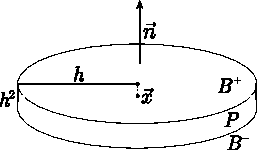
\includegraphics[width=0.6\textwidth]{images/sample.pdf}
% \caption[caption za v kazalo]{Dolg caption pod sliko}
        \caption[Primer vektorske slike.]{Primer vektorske slike z oznakami v enaki pisavi, kot jo
        uporablja \LaTeX{}. Narejena je s programom Inkscape, \LaTeX{} oznake so importane v
        Inkscape iz pomožnega PDF.}
        \label{fig:sample}
    \end{figure}

    \begin{figure}[h]
        \centering
        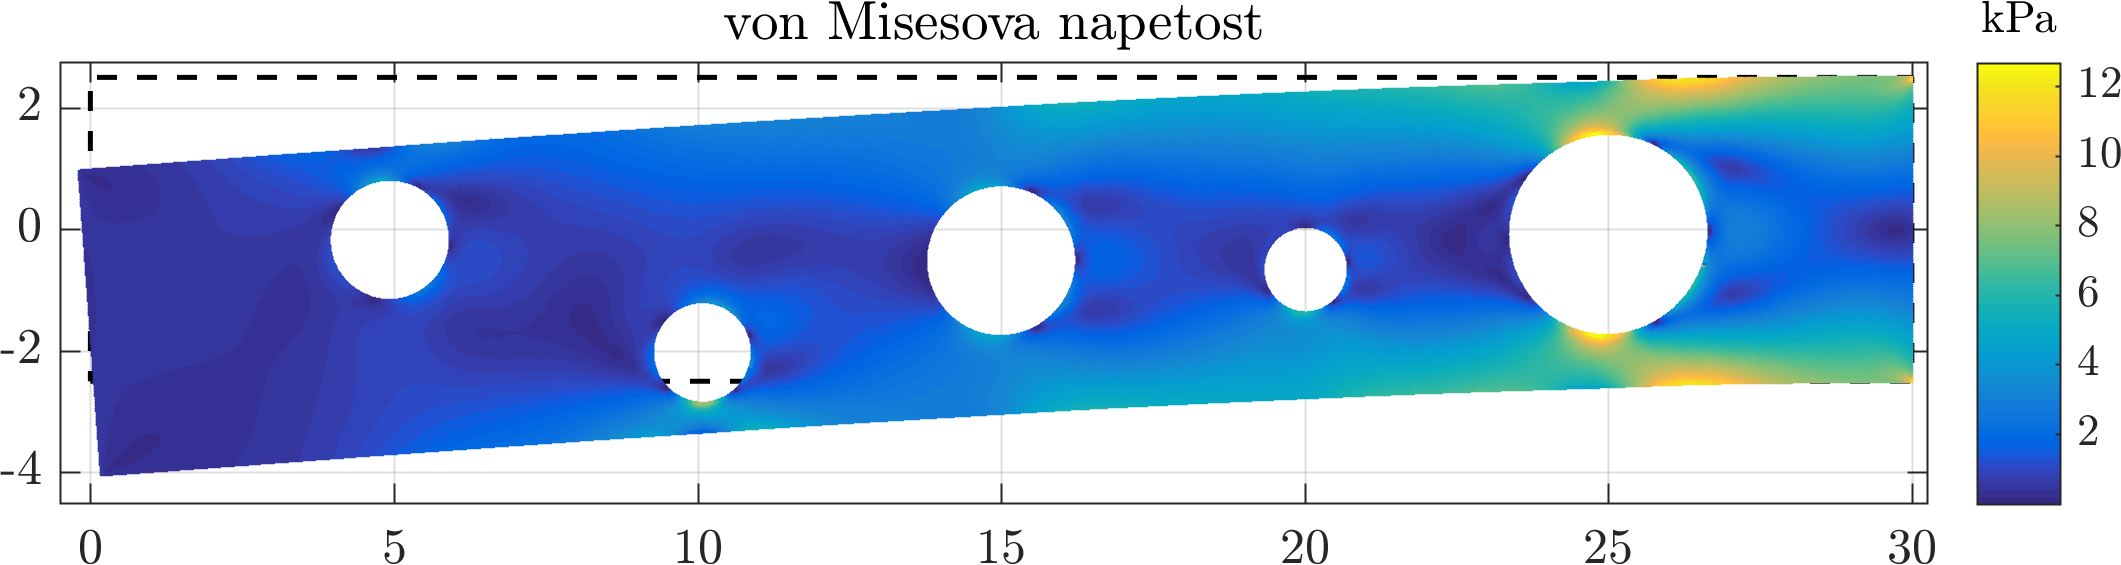
\includegraphics[width=0.8\textwidth]{images/image.png}
        \caption[Primer bitne slike.]{Primer bitne slike, izvožene iz Matlaba. Poskrbite, da so slike v
        dovolj visoki resoluciji in da ne vsebujejo prosojnih elementov (to zahteva PDF/A-1b format).}
        \label{fig:image}
    \end{figure}

    \subsection{Kako narediti stvarno kazalo}
    Dodate ukaze \verb|\index{polje}| na besede, kjer je pojavijo, kot tukaj\index{tukaj}.
    Več o stvarnih kazalih je na voljo na \url{https://en.wikibooks.org/wiki/LaTeX/Indexing}.

    \subsection{Navajanje literature}
    Članke citiramo z uporabo \verb|\cite{label}|, \verb|\cite[text]{label}| ali pa več naenkrat s
    \verb|\cite\{label1, label2}|. Tudi tukaj predhodno besedo in citat povežemo z nedeljivim presledkom
    $\sim$. Na primer~\cite{chen2006meshless,liu2001point}, ali pa \cite{kibriya2007empirical},\cite{kibriya2007empirical}, ali pa
    \cite[str.\ 12]{trobec2015parallel}, \cite[enačba (2.3)]{pereira2016convergence}.
    Vnosi iz \verb|.bib| datoteke, ki niso citirani, se ne prikažejo v seznamu literature, zato jih
    tukaj citiram.~\cite{vene2000categorical}, \cite{gregoric2017stopniceni}, \cite{slak2015induktivni},
    \cite{nsphere}, \cite{kearsley1975linearly}, \cite{STtemplate}, \cite{NunbergerTand}, \cite{vanoosten2008realizability}.

\end{document}
